\chapter{Diseño e Implementación}
\label{Chapter3}

\section{Req}

% \input{example}

\section{Infraestructura para el Desarrollo}

\subsection{Simulación}

\subsubsection{¿Qué es \textit{cocotb}?}
\textit{cocotb} (por sus siglas en inglés \textit{COroutine based COsimulation TestBench}) es
un entorno de \textit{TestBench} de verificación de simulación basado en
corrutinas para verificar RTL (por sus siglas en inglés \textit{Register Transfer Level})
descriptos en VHDL y SystemVerilog utilizando Python.

Este \textit{Framework} es completamente gratuito, de código abierto (Licencia
BSD) y alojado en GitHub. \textit{cocotb} requiere un simulador para simular el
diseño HDL (por sus siglas en inglés \textit{Hardware Description Language}) y se puede
utilizar con una variedad de simuladores en multiples sistemas operativos.

\textit{cocotb} fomenta la filosofía de reutilización de diseño y pruebas
aleatorias que UVM, sin embargo, está implementado en Python.

Con \textit{cocotb}, los HDL tradicionales se utilizan solo para el diseño en
sí, no para el banco de pruebas. Además, tiene soporte incorporado para
integrarse con sistemas de integración continua y fue diseñado específicamente
para reducir la sobrecarga de la creación de una prueba.También descubre
automáticamente las pruebas, por lo que no se requiere un paso adicional para
agregar una prueba a una regresión.

La verificación se realiza integramente con Python, lo cual tiene varias
ventajas por sobre el uso de SystemVerilog o VHDL para la verificación:

\begin{itemize}
  \item Es rápido escribir en Python, es un lenguaje muy productivo.
  \item Es fácil interfacear con otros lenguajes.
  \item Python tiene una enorme biblioteca de código existente para reutilizar.
  \item Python es interpretado: las pruebas se pueden editar y volver a ejecutar
  sin tener que recompilar el diseño.
  \item Python es popular: muchos más desarrolladores conocen Python que
  SystemVerilog o VHDL.
\end{itemize}

\subsubsection{¿Cómo funciona \textit{cocotb}?}

Un banco de pruebas típico de \textit{cocotb} no requiere código RTL adicional.
El Diseño Bajo Prueba (DUT, por sus siglas en inglés \textit{Design\/Device
under Test}) se instancía como el \textit{toplevel} en el simulador sin ningún
código que haga de interfaz o \textit{wrapper}. \textit{cocotb} proporciona
estímulos a las entradas del DUT (o incluso más abajo en la jerarquía) y
supervisa las salidas directamente desde Python.

\begin{figure}[h]
  \centering
  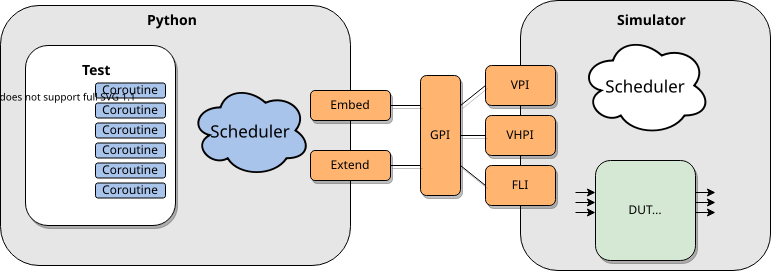
\includegraphics[width=0.7\textwidth]{./Figures/cocotb_overview.png}
  \caption{Visión general de \textit{cocotb}.}
\end{figure}

% Una prueba es simplemente una función Python. En cualquier momento, el simulador
% está avanzando en el tiempo o el código Python se está ejecutando. La palabra
% clave \texttt{await} se utiliza para indicar cuándo pasar el control de
% ejecución de vuelta al simulador. Una prueba puede generar múltiples corutinas,
% lo que permite flujos de ejecución independientes.

\subsection{CI-CD}

\section{Estructura General del Sistema}

\section{{Planificación}}
